\section{Tổng quan về mạng ad-hoc}
\label{sec:adhoc}
\subsection{Khái niệm mạng ad-hoc}

Mạng ad-hoc (Mobile Ad-hoc Network - MANET) là một loại mạng không dây phân tán, trong đó các node mạng có khả năng tự tổ chức và giao tiếp trực tiếp với nhau mà không cần sự hỗ trợ của cơ sở hạ tầng như trạm phát sóng, router hay điểm truy cập. Mỗi node trong mạng ad-hoc đóng vai trò vừa là thiết bị đầu cuối vừa là bộ định tuyến, có khả năng chuyển tiếp dữ liệu cho các node khác. Đặc điểm này giúp mạng ad-hoc có tính linh hoạt cao và phù hợp với nhiều ứng dụng trong thực tế.

\begin{figure}[h!]
    \centering
    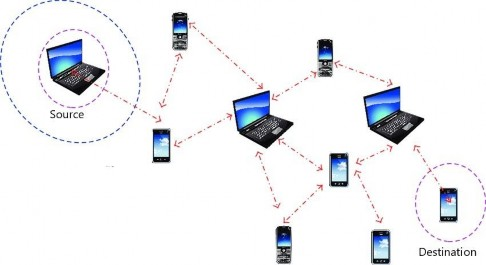
\includegraphics[width=1\textwidth]{chapter3/image/adhoc.jpg}
    \caption{Mạng ad-hoc}
   \label{fig:adhoc}
\end{figure}

Mạng ad-hoc được hình thành khi một nhóm các thiết bị không dây tự động kết nối với nhau để tạo thành một mạng tạm thời mà không cần cấu hình trước hay sự can thiệp của quản trị viên. Thuật ngữ "ad-hoc" xuất phát từ tiếng Latin, có nghĩa là "cho mục đích này" hoặc "tạm thời", phản ánh đúng bản chất linh hoạt và tự tổ chức của loại mạng này. Trong mạng ad-hoc, các node có thể tham gia hoặc rời khỏi mạng một cách tự do, dẫn đến topology mạng thay đổi liên tục theo thời gian.

\subsection{Đặc điểm của mạng ad-hoc}

Mạng ad-hoc có một số đặc điểm nổi bật phân biệt với các loại mạng truyền thống. Thứ nhất, mạng có cấu trúc phân tán (decentralized), không có node trung tâm điều khiển toàn bộ hoạt động của mạng. Thứ hai, mạng có topology thay đổi thường xuyên do các node có thể di chuyển, tham gia hoặc rời khỏi mạng bất kỳ lúc nào. Thứ ba, mạng hỗ trợ truyền thông đa chặng (multi-hop), cho phép dữ liệu được chuyển tiếp qua nhiều node trung gian để đến đích khi hai node không nằm trong phạm vi truyền thông trực tiếp. Thứ tư, các node trong mạng có tài nguyên hạn chế về năng lượng, băng thông và khả năng xử lý.

\subsection{Ứng dụng của mạng ad-hoc}

Mạng ad-hoc được ứng dụng rộng rãi trong nhiều lĩnh vực khác nhau. Trong quân sự, mạng ad-hoc cho phép các đơn vị chiến đấu duy trì liên lạc trong môi trường không có cơ sở hạ tầng viễn thông. Trong cứu hộ cứu nạn, mạng ad-hoc giúp các đội cứu hộ phối hợp hoạt động khi hệ thống thông tin liên lạc bị hư hại do thiên tai. Trong lĩnh vực Internet of Things (IoT), mạng ad-hoc được sử dụng để kết nối các thiết bị cảm biến trong các ứng dụng giám sát môi trường, nông nghiệp thông minh và quản lý tòa nhà. Ngoài ra, mạng ad-hoc còn được ứng dụng trong mạng xe cộ (Vehicular Ad-hoc Network - VANET) để hỗ trợ giao thông thông minh.

\subsection{Thách thức trong mạng ad-hoc}

Mạng ad-hoc đối mặt với nhiều thách thức kỹ thuật cần giải quyết. Thách thức đầu tiên là vấn đề định tuyến, do topology mạng thay đổi liên tục, các thuật toán định tuyến cần có khả năng thích ứng nhanh để duy trì đường truyền dữ liệu. Thách thức thứ hai là tiết kiệm năng lượng, các node thường hoạt động bằng pin nên cần tối ưu hóa việc sử dụng năng lượng trong quá trình truyền nhận và xử lý dữ liệu. Thách thức thứ ba là bảo mật, do không có cơ sở hạ tầng tập trung, việc xác thực và mã hóa trở nên phức tạp hơn. Thách thức thứ tư là chất lượng dịch vụ (Quality of Service - QoS), việc đảm bảo độ trễ thấp và tỷ lệ mất gói tin nhỏ trong môi trường mạng động là một bài toán khó. Những thách thức này đặt ra yêu cầu cho việc nghiên cứu và phát triển các giải pháp định tuyến hiệu quả, trong đó thuật toán định tuyến dựa trên Gradient là một hướng tiếp cận tiềm năng.
